\documentclass[12pt,a4paper]{report}

\usepackage[margin=1in]{geometry}
\usepackage[table]{xcolor}
\usepackage{array}
\usepackage{booktabs}
\usepackage{longtable}
\usepackage{setspace}
\usepackage{hyperref}
\usepackage{fancyhdr}
\usepackage{titlesec}
\usepackage{enumitem}
\usepackage{tikz}
\usetikzlibrary{arrows.meta,positioning,shapes.geometric}

\definecolor{primary}{HTML}{FF3E41}
\definecolor{secondary}{HTML}{00A9FF}
\definecolor{dark}{HTML}{060315}
\definecolor{soft}{HTML}{F7FBFF}
\definecolor{linegray}{HTML}{D9E2EC}

\hypersetup{
    colorlinks=true,
    linkcolor=dark,
    urlcolor=secondary,
    citecolor=primary
}

\pagestyle{fancy}
\fancyhf{}
\lhead{\textbf{Logistica Project Report}}
\rhead{\thepage}
\renewcommand{\headrulewidth}{0.4pt}

\titleformat{\chapter}{\normalfont\huge\bfseries\color{dark}}{\thechapter.}{0.5em}{}
\titleformat{\section}{\normalfont\Large\bfseries\color{dark}}{\thesection}{0.5em}{}
\titleformat{\subsection}{\normalfont\large\bfseries\color{dark}}{\thesubsection}{0.5em}{}
\setlist[itemize]{noitemsep, topsep=4pt}
\setstretch{1.18}

\newcommand{\project}{Logistica}
\newcolumntype{L}[1]{>{\raggedright\arraybackslash}p{#1}}

\begin{document}

\begin{titlepage}
    \centering
    \vspace*{1.5cm}
    {\Huge\bfseries\color{dark} Professional Project Report\par}
    \vspace{0.4cm}
    {\LARGE\bfseries\color{primary} \project: Logistics Service Booking System\par}
    \vspace{1.2cm}
    {\large A Laravel-based web application for public service browsing, customer booking, and administrative order management.\par}
    \vfill
    \begin{tabular}{rl}
        \textbf{Project Name:} & \project \\
        \textbf{Application Type:} & Web-based logistics booking and management system \\
        \textbf{Framework:} & Laravel 12 \\
        \textbf{Database:} & MySQL \\
        \textbf{Report Date:} & May 23, 2026 \\
    \end{tabular}
    \vfill
    {\large Prepared for academic and technical presentation use\par}
\end{titlepage}

\tableofcontents
\newpage

\chapter*{Executive Summary}
\addcontentsline{toc}{chapter}{Executive Summary}

\project{} is a professional logistics service booking platform built with Laravel. The application allows visitors to browse company information and available logistics services, registered customers to create shipment booking requests, and administrators to manage services, users, and booking decisions from a secured dashboard. The system follows Laravel's MVC architecture: Blade templates render the frontend, named routes connect user actions to controllers, Form Request classes validate critical operations, Eloquent models communicate with the MySQL database, and middleware protects authenticated and admin-only areas.

The main business workflow starts when an administrator publishes active logistics services. Customers can then select a service, submit pickup and delivery details, and track the request status from their dashboard. Admin users review each booking, set its status to pending, accepted, or rejected, and optionally provide an admin note. The updated decision is immediately visible in the user's booking records.

\chapter{Project Overview}

\section{Purpose}

The purpose of \project{} is to digitize a logistics company's service discovery and booking workflow. Instead of relying only on static pages, the application connects service listings, user accounts, booking forms, and administrative review into one database-backed system.

\section{Core Objectives}

\begin{itemize}
    \item Present a polished public website for a logistics company.
    \item Allow customers to register, log in, and submit service bookings.
    \item Allow administrators to create, update, deactivate, and delete services when safe.
    \item Allow administrators to review booking requests and update their status.
    \item Keep customer booking history visible in the user dashboard.
    \item Protect sensitive operations using authentication, CSRF protection, validation, and admin middleware.
\end{itemize}

\section{User Roles}

\begin{longtable}{L{0.22\textwidth} L{0.68\textwidth}}
\toprule
\textbf{Role} & \textbf{Capabilities} \\
\midrule
Guest Visitor & Can view public pages such as Home, About, Services, Features, Contact, Login, and Register. Booking actions redirect to authentication when required. \\
Customer User & Can access the user dashboard, view active services, submit bookings, and track booking statuses and admin notes. \\
Administrator & Can access the admin dashboard, manage logistics services, view users, inspect analytics, and accept or reject booking requests. \\
\bottomrule
\end{longtable}

\chapter{Technology Stack}

\section{Backend Technologies}

\begin{longtable}{L{0.28\textwidth} L{0.62\textwidth}}
\toprule
\textbf{Technology} & \textbf{Use in Project} \\
\midrule
PHP 8.2 & Primary server-side programming language. \\
Laravel 12.60.2 & Main backend framework for routing, controllers, middleware, validation, sessions, authentication, and MVC structure. \\
Laravel Eloquent ORM & Maps application models to database tables such as users, logistics services, and service orders. \\
MySQL & Relational database engine used for users, services, bookings, sessions, cache, and jobs. \\
Laravel Form Requests & Used for booking submission validation and booking status update validation. \\
Laravel Middleware & Used for authentication and admin-only access control. \\
Laravel Blade & Server-side templating engine used to render public pages, authentication pages, dashboards, and forms. \\
\bottomrule
\end{longtable}

\section{Frontend Technologies}

\begin{longtable}{L{0.28\textwidth} L{0.62\textwidth}}
\toprule
\textbf{Technology} & \textbf{Use in Project} \\
\midrule
HTML5 and CSS3 & Structure and custom visual styling of all pages. \\
Bootstrap 5 & Responsive grid, navbar, forms, buttons, tables, and layout utilities. \\
Font Awesome and Bootstrap Icons & Icon system for services, dashboards, navigation, and action buttons. \\
jQuery & Supports frontend template interactions and plugin behavior. \\
Owl Carousel & Powers the homepage carousel. \\
WOW.js and Animate.css & Adds scroll and entrance animations. \\
SweetAlert2 & Displays success, warning, error, validation, and delete-confirmation alerts. \\
JavaScript LocalStorage & Stores the selected theme preference for light, dark, ocean, forest, and sunset modes. \\
Vite and Tailwind CSS 4 & Present in the project toolchain for modern asset bundling and CSS workflow support. \\
\bottomrule
\end{longtable}

\section{Testing and Tooling}

\begin{longtable}{L{0.28\textwidth} L{0.62\textwidth}}
\toprule
\textbf{Tool} & \textbf{Use in Project} \\
\midrule
Pest 3 & Feature testing framework used to verify authentication, routing, booking, and admin flows. \\
PHPUnit 11 & Underlying PHP test runner used by Pest. \\
Laravel Pint & Code formatting tool for Laravel/PHP style consistency. \\
Composer & PHP dependency manager and script runner. \\
npm & JavaScript dependency manager for Vite and frontend tooling. \\
\bottomrule
\end{longtable}

\chapter{System Architecture}

\section{Architectural Pattern}

\project{} follows the Model-View-Controller pattern used by Laravel applications.

\begin{itemize}
    \item \textbf{Models} represent data entities and relationships: \texttt{User}, \texttt{LogisticsService}, and \texttt{ServiceOrder}.
    \item \textbf{Views} are Blade templates located in \texttt{resources/views}. They render public pages, forms, dashboards, and records.
    \item \textbf{Controllers} receive routed requests, run business logic, read or write models, and return views or redirects.
    \item \textbf{Routes} in \texttt{routes/web.php} define the URL, HTTP method, route name, middleware, and controller action.
    \item \textbf{Middleware} protects authenticated pages and admin-only pages.
    \item \textbf{Form Requests} centralize validation and authorization for important write operations.
\end{itemize}

\section{Request Lifecycle}

\begin{center}
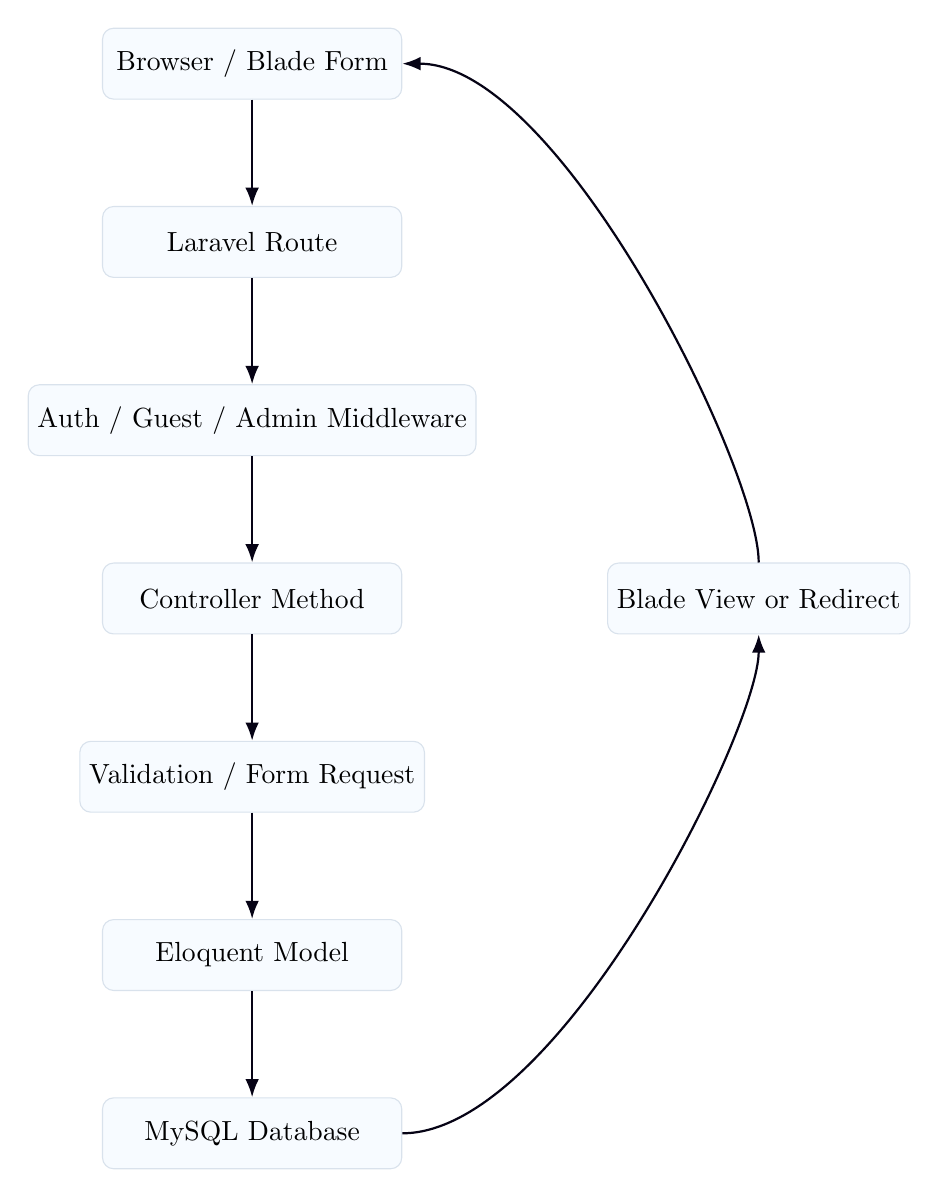
\begin{tikzpicture}[
    node distance=1.35cm,
    box/.style={rectangle, draw=linegray, fill=soft, rounded corners, minimum width=3.8cm, minimum height=0.9cm, align=center},
    arrow/.style={-Latex, thick, color=dark}
]
\node[box] (browser) {Browser / Blade Form};
\node[box, below=of browser] (route) {Laravel Route};
\node[box, below=of route] (middleware) {Auth / Guest / Admin Middleware};
\node[box, below=of middleware] (controller) {Controller Method};
\node[box, below=of controller] (request) {Validation / Form Request};
\node[box, below=of request] (model) {Eloquent Model};
\node[box, below=of model] (db) {MySQL Database};
\node[box, right=2.6cm of controller] (response) {Blade View or Redirect};

\draw[arrow] (browser) -- (route);
\draw[arrow] (route) -- (middleware);
\draw[arrow] (middleware) -- (controller);
\draw[arrow] (controller) -- (request);
\draw[arrow] (request) -- (model);
\draw[arrow] (model) -- (db);
\draw[arrow] (db.east) .. controls +(2,0) and +(0,-1.2) .. (response.south);
\draw[arrow] (response.north) .. controls +(0,1.2) and +(2,0) .. (browser.east);
\end{tikzpicture}
\end{center}

\section{Project Structure}

\begin{longtable}{L{0.33\textwidth} L{0.57\textwidth}}
\toprule
\textbf{Path} & \textbf{Responsibility} \\
\midrule
\texttt{routes/web.php} & Defines public, guest, authenticated, and admin web routes. \\
\texttt{app/Http/Controllers} & Contains controllers for pages, authentication, dashboards, user bookings, and admin operations. \\
\texttt{app/Http/Requests} & Contains validation and authorization classes for booking creation and booking status updates. \\
\texttt{app/Models} & Contains Eloquent models and relationships. \\
\texttt{app/Http/Middleware} & Contains the custom admin-access middleware. \\
\texttt{resources/views} & Contains Blade templates for public pages, auth pages, user dashboard, admin dashboard, and booking forms. \\
\texttt{database/migrations} & Defines database schema for users, services, service orders, cache, sessions, and jobs. \\
\texttt{tests/Feature} & Contains Pest feature tests for authentication, booking, and admin workflows. \\
\texttt{public} & Stores frontend assets such as images, Bootstrap CSS, custom CSS, JavaScript, and plugin files. \\
\bottomrule
\end{longtable}

\chapter{Database Design}

\section{Main Tables}

\begin{longtable}{L{0.28\textwidth} L{0.62\textwidth}}
\toprule
\textbf{Table} & \textbf{Purpose} \\
\midrule
\texttt{users} & Stores customer and admin accounts. Important fields include \texttt{name}, \texttt{email}, \texttt{phone}, \texttt{password}, and \texttt{is\_admin}. \\
\texttt{logistics\_services} & Stores service listings managed by admins. Important fields include \texttt{name}, \texttt{icon}, \texttt{image\_path}, \texttt{link\_url}, \texttt{description}, \texttt{base\_price}, \texttt{is\_active}, and \texttt{sort\_order}. \\
\texttt{service\_orders} & Stores customer booking requests. Important fields include \texttt{user\_id}, \texttt{logistics\_service\_id}, \texttt{status}, pickup and delivery details, notes, reviewer, and review timestamp. \\
\texttt{sessions} & Stores session data for logged-in users. \\
\texttt{cache}, \texttt{jobs}, and related tables & Support Laravel cache, queue, and background job infrastructure. \\
\bottomrule
\end{longtable}

\section{Entity Relationships}

\begin{itemize}
    \item A \texttt{User} has many \texttt{ServiceOrder} records.
    \item A \texttt{LogisticsService} has many \texttt{ServiceOrder} records.
    \item A \texttt{ServiceOrder} belongs to one customer user.
    \item A \texttt{ServiceOrder} belongs to one logistics service.
    \item A \texttt{ServiceOrder} may belong to one admin reviewer through the \texttt{reviewed\_by} field.
\end{itemize}

\begin{center}
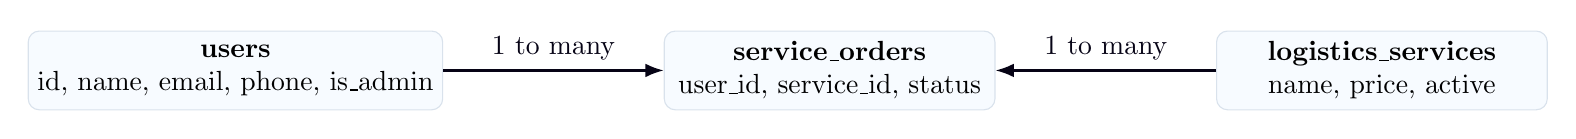
\begin{tikzpicture}[
    table/.style={rectangle, draw=linegray, fill=soft, rounded corners, minimum width=4.2cm, minimum height=1.0cm, align=center},
    arrow/.style={-Latex, thick, color=dark}
]
\node[table] (users) {\textbf{users}\\id, name, email, phone, is\_admin};
\node[table, right=2.8cm of users] (orders) {\textbf{service\_orders}\\user\_id, service\_id, status};
\node[table, right=2.8cm of orders] (services) {\textbf{logistics\_services}\\name, price, active};
\draw[arrow] (users) -- node[above]{1 to many} (orders);
\draw[arrow] (services) -- node[above]{1 to many} (orders);
\end{tikzpicture}
\end{center}

\chapter{Functional Modules}

\section{Public Website Module}

The public website uses Blade pages such as \texttt{index.blade.php}, \texttt{about.blade.php}, \texttt{service.blade.php}, \texttt{feature.blade.php}, and \texttt{contact.blade.php}. These pages are served by \texttt{PageController}. The Home and Services pages load active services from \texttt{LogisticsService} so that public service cards reflect records controlled by the admin dashboard.

\section{Authentication Module}

The authentication module uses one login system for both users and admins. During login, \texttt{AuthController@login} validates credentials, attempts authentication, regenerates the session, and redirects users according to \texttt{users.is\_admin}. Admin accounts go to the admin dashboard, while normal users go to the user dashboard.

Registration validates name, email, phone, password, and password confirmation. New users are stored through the \texttt{User} model. The model casts the password as \texttt{hashed}, so Laravel hashes the password before saving it.

\section{Customer Booking Module}

Customers can create bookings from the homepage booking form, the Bookings page, the User Dashboard, or a selected service page. All of these forms submit to the same backend endpoint: \texttt{user.orders.store}. The \texttt{StoreBookingRequest} validates that the selected service exists and is active, validates pickup and delivery addresses, checks date and weight rules, and authorizes only normal authenticated users.

After validation, \texttt{UserDashboardController@storeOrder} creates a \texttt{ServiceOrder} with status \texttt{pending}. The user is redirected to the dashboard, where the new booking appears in the Records section.

\section{Admin Management Module}

The admin dashboard is protected by the \texttt{auth} middleware and a custom \texttt{admin} middleware. Admins can add services, edit service details, toggle active status, delete services without attached orders, view users, inspect basic analytics, and update booking decisions.

When an admin updates a booking, \texttt{UpdateBookingStatusRequest} verifies that the user is an admin and that the selected status is one of \texttt{pending}, \texttt{accepted}, or \texttt{rejected}. The controller saves the decision, admin note, reviewer ID, and review timestamp. The user's dashboard then displays the updated status and note.

\chapter{Frontend Action to Backend Mapping}

\rowcolors{2}{soft}{white}
\begin{longtable}{L{0.20\textwidth} L{0.20\textwidth} L{0.20\textwidth} L{0.30\textwidth}}
\toprule
\textbf{Frontend Action} & \textbf{Route / Method} & \textbf{Controller} & \textbf{Backend Result} \\
\midrule
\endhead
Click Home in navbar & \texttt{GET /} & \texttt{PageController@home} & Loads the homepage and passes up to six active services to the view. \\
Click About & \texttt{GET /about} & \texttt{PageController@about} & Renders the About page. \\
Click Services & \texttt{GET /service} & \texttt{PageController@service} & Loads all active services ordered by sort order and name. \\
Click Features & \texttt{GET /feature} & \texttt{PageController@feature} & Renders the Features page. \\
Click Contact & \texttt{GET /contact} & \texttt{PageController@contact} & Renders the Contact page. The visible contact form is static and has no storage backend in the current project. \\
Click Book Now from homepage hero & \texttt{GET /bookings} & \texttt{UserDashboardController@bookings} & Requires login. Shows the booking page with active services and the user's latest bookings. \\
Click Book Now on a service card & \texttt{GET /services/\{service\}/order} & \texttt{UserDashboardController@createOrder} & Uses route model binding to load the selected service. If active, it renders a preselected booking form. \\
Submit login form & \texttt{POST /login} & \texttt{AuthController@login} & Validates credentials, authenticates the user, regenerates session, and redirects by role. \\
Submit register form & \texttt{POST /register} & \texttt{AuthController@register} & Validates account details, creates a user, logs the user in, and redirects to the user dashboard. \\
Submit logout form & \texttt{POST /logout} & \texttt{AuthController@logout} & Logs the user out, invalidates session, regenerates CSRF token, and redirects home. \\
Submit user booking form & \texttt{POST /user/service-orders} & \texttt{UserDashboardController@storeOrder} & Validates booking data, creates a pending service order, and redirects to the user dashboard. \\
Open dashboard route & \texttt{GET /dashboard} & \texttt{DashboardController} & Redirects admins to \texttt{admin.dashboard} and customers to \texttt{user.dashboard}. \\
Open user dashboard & \texttt{GET /user/dashboard} & \texttt{UserDashboardController@dashboard} & Loads active services and the logged-in user's service orders. Admins are redirected to the admin dashboard. \\
Open admin dashboard & \texttt{GET /admin/dashboard} & \texttt{AdminController@dashboard} & Loads services, orders, users, service image options, and dashboard statistics. \\
Add a service & \texttt{POST /admin/services} & \texttt{AdminController@storeService} & Validates service data and creates a new logistics service. \\
Edit a service & \texttt{PATCH /admin/services/\{service\}} & \texttt{AdminController@updateService} & Updates service name, icon, image, link, description, base price, active status, and sort order. \\
Delete a service & \texttt{DELETE /admin/services/\{service\}} & \texttt{AdminController@destroyService} & Deletes the service only when no orders exist for it. Otherwise, deletion is blocked. \\
Update booking decision & \texttt{PATCH /admin/service-orders/\{order\}/status} & \texttt{AdminController@updateOrderStatus} & Saves status, admin note, reviewer ID, and review timestamp. \\
Change website theme & Frontend JavaScript only & No controller & Updates \texttt{data-theme} and stores the selected theme in browser localStorage. \\
Click dashboard side menu & Frontend anchor links & No controller & Scrolls within the dashboard and changes the active menu state using JavaScript. \\
Confirm service deletion & Frontend JavaScript + DELETE route & \texttt{AdminController@destroyService} & SweetAlert2 asks for confirmation, then submits the protected delete form if confirmed. \\
\bottomrule
\end{longtable}

\chapter{Security, Validation, and Access Control}

\section{Authentication and Authorization}

Authenticated routes are grouped under Laravel's \texttt{auth} middleware. Guest-only routes such as login and registration are grouped under \texttt{guest}. Admin routes are nested under \texttt{auth} and the custom \texttt{admin} middleware, which checks whether the logged-in user has \texttt{is\_admin = true}. If a non-admin tries to access admin pages, the middleware logs them out, invalidates the session, regenerates the token, and redirects to login.

\section{CSRF Protection}

All write forms include Blade's \texttt{@csrf} directive. This protects POST, PATCH, and DELETE actions from cross-site request forgery attacks.

\section{Validation}

The system validates both customer and admin inputs:

\begin{itemize}
    \item Login requires a valid email and password.
    \item Registration requires unique email and phone values, a name, and a confirmed password with a minimum length of eight characters.
    \item Booking creation requires an active logistics service, pickup address, delivery address, optional future date, optional package weight, and optional note.
    \item Admin booking decisions require a valid status from the allowed status list.
    \item Admin service management validates service name, icon, image path, link URL, description, price, active flag, and sort order.
\end{itemize}

\section{Data Protection}

The \texttt{User} model hides passwords and remember tokens from serialization. Passwords are hashed automatically through Laravel's \texttt{hashed} cast. The system also protects historical booking records by preventing admins from deleting services that already have attached orders.

\chapter{Testing Coverage}

The project includes Pest feature tests in \texttt{tests/Feature/AuthFlowTest.php}. These tests cover important user journeys:

\begin{itemize}
    \item Login and registration pages render correctly.
    \item New accounts are created as normal users.
    \item Login redirects users based on the \texttt{is\_admin} boolean.
    \item Booking pages require authentication.
    \item Old quote links redirect to the authenticated booking route.
    \item Service booking links preserve the intended destination after login.
    \item Authenticated users can book a selected service.
    \item Normal users cannot enter the admin dashboard.
    \item Admin service creation and booking decisions appear in the user dashboard.
    \item Admins can delete services without orders.
    \item Admins cannot delete services that already have orders.
\end{itemize}

\chapter{Deployment and Running the Project}

\section{Local Setup}

A typical local setup follows these steps:

\begin{enumerate}
    \item Install PHP dependencies with \texttt{composer install}.
    \item Create the environment file from \texttt{.env.example}.
    \item Generate the Laravel application key with \texttt{php artisan key:generate}.
    \item Configure MySQL credentials in \texttt{.env}.
    \item Run migrations with \texttt{php artisan migrate}.
    \item Install frontend dependencies with \texttt{npm install}.
    \item Build assets with \texttt{npm run build}, or run Vite during development with \texttt{npm run dev}.
    \item Start the Laravel server with \texttt{php artisan serve}, or use the project's \texttt{composer run dev} script for the server, queue listener, and Vite together.
\end{enumerate}

\section{Production Notes}

For production, the application should use a configured web server, a production MySQL database, cached configuration, migrated database schema, built frontend assets, and secure environment variables. Laravel Cloud, a VPS, or a managed PHP hosting environment can be used depending on project requirements.

\chapter{Conclusion}

\project{} is a complete Laravel-based logistics booking system with a clear separation between public content, authenticated customer actions, and protected administrator operations. The application demonstrates practical use of Laravel routing, Blade views, Eloquent models, Form Requests, middleware, MySQL persistence, and Pest feature testing. Its core workflow is direct and maintainable: admins publish services, users submit bookings, admins review requests, and users track the resulting status from their dashboard.

The project is suitable for presentation as a professional academic or portfolio system because it includes visible business functionality, structured backend flow, role-based access control, database relationships, and test coverage for the most important behaviors.

\end{document}
